% Chapter 4

\chapter{Experiments and Results} % Main chapter title

\label{Chapter4} %

In this chapter, we describe the experiments we ran to verify the functionality of the proposed framework. We also compare different the different implementation alternatives taking kernel execution time as our main metric. All of our experiments are run on the Nallatech 510T Compute Accelerator card which contains an Alterra Arria 10 1150 GX FPGA. Our kernels are compiled with the Intel OpenCL SDK with Quartus 17.1. The host program is compiled with gcc v.7.2.0. All of the tools that support the development workflow were tested using Python 3.6.5. 
The model we use for training and inference is the LeNet discussed in section \ref{lenetpilot}.


%----------------------------------------------------------------------------------------
\section{Convolution Implementations}

\begin{table}[]
\centering
\begin{tabular}{|l|l|}
\hline
\textbf{Parameter}    & \textbf{Value} \\ \hline
Image                 & 100x100        \\ \hline
Filter                & 3x3            \\ \hline
Input/Output Channels & 1              \\ \hline
\end{tabular}
\caption{Configuration for the Part I Test Case}
\label{tab:partoneconfig}
\end{table}

\subsection{Part I : Simple Example} \label{testone}
In this section, we compare the different convolution implementations. Those are the simple implementation, sliding buffer, and row-stationary \ref{rowimpl}. The parameters are shown in Table \ref{tab:partoneconfig}. 

\begin{figure}[h]
\centering
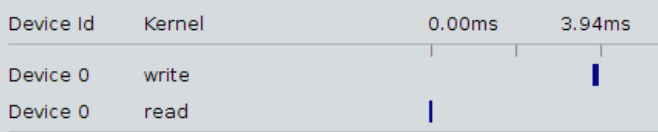
\includegraphics[width=0.7\textwidth]{Figures/profilerow}
\decoRule
\caption[profilerow]{ Dynamic Profiling result for row-stationary Implementation}
\label{fig:rowstatp}
\end{figure}

\begin{table}[]
\centering
\begin{tabular}{|l|c|c|}
\hline
\textbf{Implementation}        & \multicolumn{1}{l|}{\textbf{Execution Time (ms)}} & \multicolumn{1}{l|}{Frequency (MHz)} \\ \hline
\textit{Simple Implementation} & 0.15                                              & 256.1                                \\ \hline
\textit{Sliding Buffer}        & 0.09                                              & 252.8                                \\ \hline
\textit{Row Stationary}        & 3.94                                              & 184.4                                \\ \hline
\end{tabular}
\caption{Results of Part I Test}
\label{tab:resultpartone}
\end{table}

The profiling results and operating frequency of the board for each of the implementations is shown in table \ref{tab:resultpartone}. In the case of the row-stationary implementation, the compute array of processing elements are \emph{autorun} kernels. Therefore they are considered to be running the whole time during execution and will not be caught by the Intel Dynamic Profiler. To approximate the time consumed we take the time difference between the reader and writer kernels that communicate with the grid as the execution time.
Unsurprisingly, the row-stationary implementation is the slowest in a small example. One reason is a low operating frequency due to a long critical path of execution. Another reason is the synchronization and communication overhead between the processing elements in the processing grid. We see also that the sliding buffer has the best performance in the case of a single large image which also makes sense. In the next section we abandon the row-stationary implementation and test the two other kernels in a real-case scenario.


\subsection{Part II : Performance in a Real-Case} 

In \ref{testone} we used a very simple two dimensional convolution to benchmark three different convolution operators. Our row-stationary implementation doesn't support a real-case convolution with multiple input and output channels. For that we compare the two other implementations ( sliding buffer, and optimized implementation \ref{slidingimpl}) configured for a large batch of size of $ 2048 $ and for a convolution requiring multiple input and output channels. This allows us to better compare both operators and to choose which one is more suitable for the LeNet model.

\begin{table}[]
\centering
\begin{tabular}{|l|l|}
\hline
\textbf{Parameter} & \textbf{Value} \\ \hline
Image              & 100x20          \\ \hline
Filter             & 5x5            \\ \hline
Input Channels     & 2             \\ \hline
Output Channels    & 6             \\ \hline
Batch Size         & 2048           \\ \hline
\end{tabular}
\caption{Configuration for Part II Test}
\label{tab:l3params}
\end{table}

\begin{table}[]
\begin{tabular}{|l|l|l|l|l|}
\hline
\textbf{Implementation}     & \textbf{Total Time (s)} & \textbf{Frequency (MHz)} & \textbf{RAMS} & \textbf{DSP} \\ \hline
\textit{Simple Convolution} & 5.37                    & 232.7                    & 85            & 4            \\ \hline
\textit{Sliding Buffer}     & 3.53                    & 65.1                     & 116           & 51           \\ \hline
\end{tabular}
\caption{Simulation Results of Different Convolution Implementations }
\label{tab:resultparttw}
\end{table}

The results are shown in Table \ref{tab:resultparttw}. The sliding buffer is faster in practice, however it comes at the expense of more resources and a lower operating frequency. This may be feasible if we only implement the convolution operation, however in the context of a neural network, we chose the first implementation as we wish to fit more network layers in the same binary. The compiled version of the simple implementation differs from that in reference section as we have removed unrolling factors to lower the resource utilization even more. We have found that kernels with resource utilization >50\% take more than 12 hours to compile and we were unable to run the full compilations without timeouts, memory limits exceeded, and placement errors. 

The results are fully pipelined for the batch of images and conform to the theoretical estimate for performance. As compute time for the convolution diminishes the effect of buffering kernel coefficients, we estimate the performance taking into consideration only the main computation loop. For the simple implementation, the calculation is as follows : \newline Number of cycles = batch size * input ch * output ch * img height * img width * filter height * filter width  = $2048 * 2 * 6 * 100 * 20 * 5 * 5 $ = 1,228,800,000 cycles. 

The frequency of operation is $232.7$ MHz, so we can estimate the time to be 5.28 seconds.
\begin{equation}
 Total Time = \frac{Number of cycles}{Frequency} = \frac{1,288,800,000}{232,700,000}  \approx 5.28 sec
\end{equation}
This theoretical calculation matches the experimental results. The same calculation can be performed to the case of the sliding buffer implementation. We note that unrolling factors in the sliding buffer reduce the number of cycles, however this is matched by a lower operating frequency as well.




%----------------------------------------------------------------------------------------
\section{Pipelined vs. Non-Pipelined Inference}

In this example we study the effect of pipelining on the inference phase of the neural network. We test both a pipelined implementation of LeNet \ref{lenetpilot} where kernels are connected by Intel OpenCL Channels and the kernels follow a sliding buffer/streamlined implementation. We also test a non-pipelined version shown in \ref{fig:comm}, where the operators are run sequentially, communicate through global memory, and exhibit different types of parallelism. The batch size is configurable at run-time, so we test the time it takes for the inference of a single image and the time for a batch of 2048 images. 

The results are that the pipelined version is effectively faster than the non-pipelined version during inference. Fig. \ref{fig:pipesingle} shows the dynamic profiler results. We note that the kernels were enqueued into separate queues and also in reverse order in the host program. This is why it seems that the softmax kernel has been running the longest, but effectively it only runs after all of the layers have been completed. We noticed that running the kernels in the order that they are supposed to execute introduced latencies due to context switching and the overhead of enqueuing the tasks from the host-side, so this reverse order gives a more accurate representation of effective time taken for inference. 

The kernels communicate through channels so we are sure that they are synchronized and the results are verified for correctness by using a LeNet CPU implementation configured with the same weights. The kernel also \emph{effectively} starts running after the reader kernel starts (which is at 0.3 ms from the initial start time because it is the last to be launched and all other layers depend on its input). 

The estimation is further verified by running the pipeline to classify a set of 2048 images and the total time taken in that case is 6.12 seconds. A simple calculation in \ref{eqn:check} shows that the theoretical results agree with the experimental results. The dynamic profiler result in \ref{fig:pipebatch} shows that all layers are being effectively utilized in case of batch image inference. 
\begin{equation}
\text{Total time = time for single image * batch size} = 0.03 * 2048 \approx 6.14\text{ seconds}
\label{eqn:check}
\end{equation}

As for the non-pipelined version, we see in \ref{fig:nonpipesingle} that in the case of inference for a single image,  the total time taken for inference is 21.53 milliseconds. Moreover, the effective time by summing up the individual kernel execution times is much less. The reason for the delay in launching kernels is mainly synchronization constructs by calling \emph{clFinish(queue)} in between kernel launches. Summing up individual kernel times leads to an effective execution time of 5.4 milliseconds. This is still significantly slower than the pipelined implementation. For inference of the batch, the effect of synchronization is minimized and we find that the total time of 11.15 seconds meets the theoretical results \ref{eqn:effect}.

\begin{equation}
\begin{array}{l}

\text{Batch Execution time = batch size * effective time one image} \\
  \text{        } = 2048 * 0.054 sec \approx 11.05 sec
\end{array}
\label{eqn:effect}
\end{equation}


\begin{table}[]
\begin{tabular}{|l|l|l|}
\hline
Implementation               & \textbf{Single Image (Effective)} & \textbf{Batch of 2048 Images} \\ \hline
\textit{Pipelined LeNet}     & 0.0033 ( 0.003 )                 & 6.12                          \\ \hline
\textit{Non-Pipelined Lenet} & 0.021 ( 0.0054 )                  & 11.15                         \\ \hline
\end{tabular}
\caption{Inference time for pipelined and non-pipelined implementations of Lenet in seconds. }
\label{tab:resultinf}
\end{table}

\begin{figure}[h!]
\centering
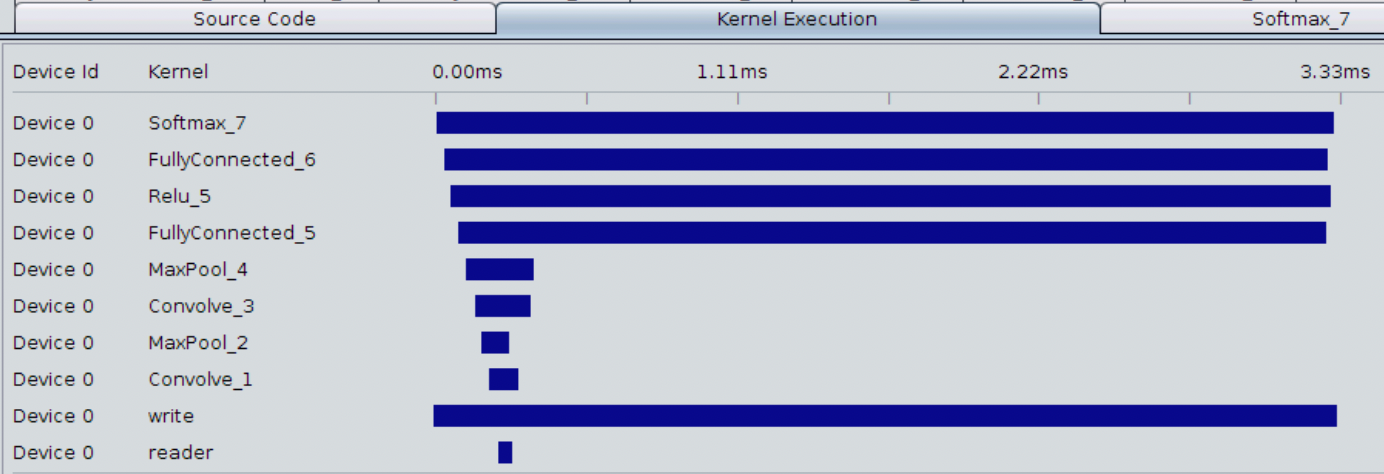
\includegraphics[width=0.85\textwidth]{Figures/pipesingle}
\decoRule
\caption[pipesingle]{ Execution time for inference of a single image (pipelined)}
\label{fig:pipesingle}
\end{figure}

\begin{figure}[h!]
\centering
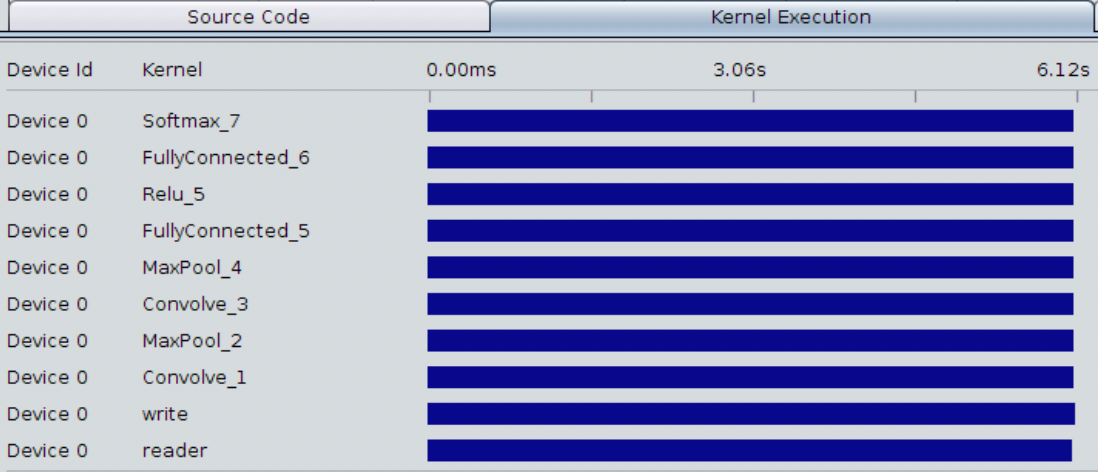
\includegraphics[width=0.85\textwidth]{Figures/pipebatch}
\decoRule
\caption[pipebatch]{ Execution time for inference of a batch of images (pipelined)}
\label{fig:pipebatch}
\end{figure}

\begin{figure}[h!]
\centering
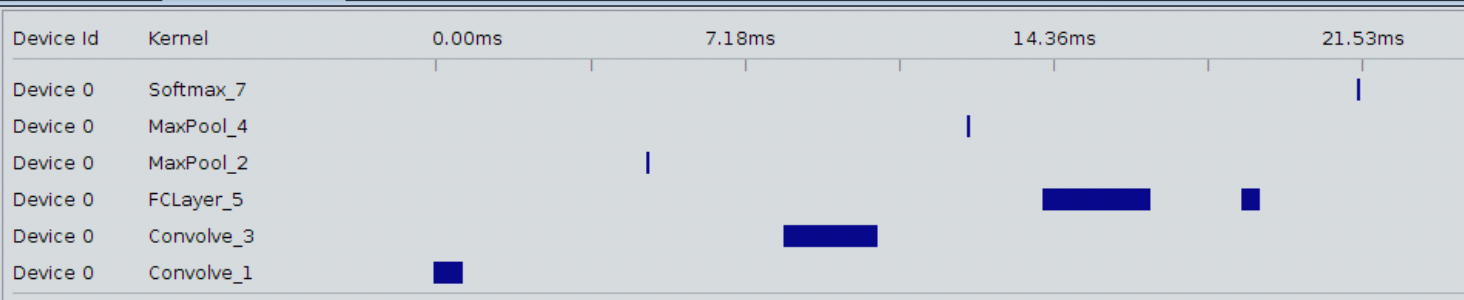
\includegraphics[width=0.85\textwidth]{Figures/nonpipesingle}
\decoRule
\caption[nonpipesingle]{ Execution time for inference of a single image (non-pipelined)}
\label{fig:nonpipesingle}
\end{figure}

\begin{figure}[h!]
\centering
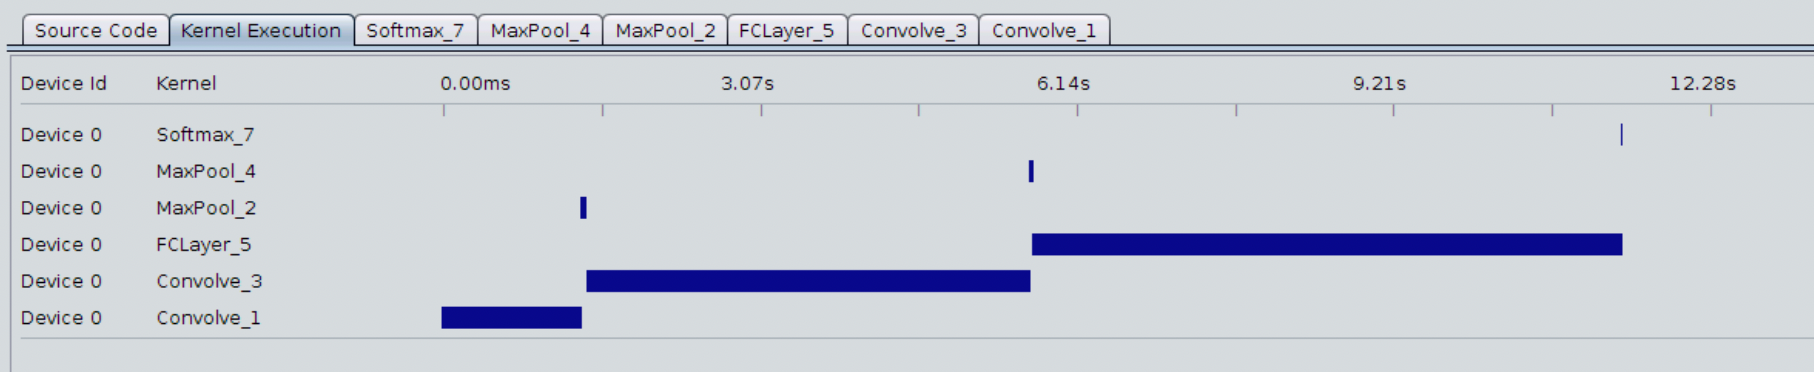
\includegraphics[width=0.85\textwidth]{Figures/nonpipebatch}
\decoRule
\caption[nonpipebatch]{ Execution time for inference of a batch of images (non-pipelined)}
\label{fig:nonpipebatch}
\end{figure}

%----------------------------------------------------------------------------------------

\newpage
\section{Training LeNet}

\subsection{Reconfiguration Time}

We implemented full minibatch backpropagation for the LeNet model. The problem we faced is that the fully optimized kernel implementations for the forward and backward propagation do not fit in a single binary. The estimated area usage was always within the Arria 10's available resources and even less than 80\% logic utilization. However, the compiler would run out of memory or crash with random error messages during compilation after tens of hours of running. For that we chose to simplify the design and break it up into a binary for forward propagation and a binary for backpropagation. The FPGA would reconfigure when switching between the two modes and in this section we evaluate the feasibility of this appraoch.

\begin{figure}[h!]
\centering
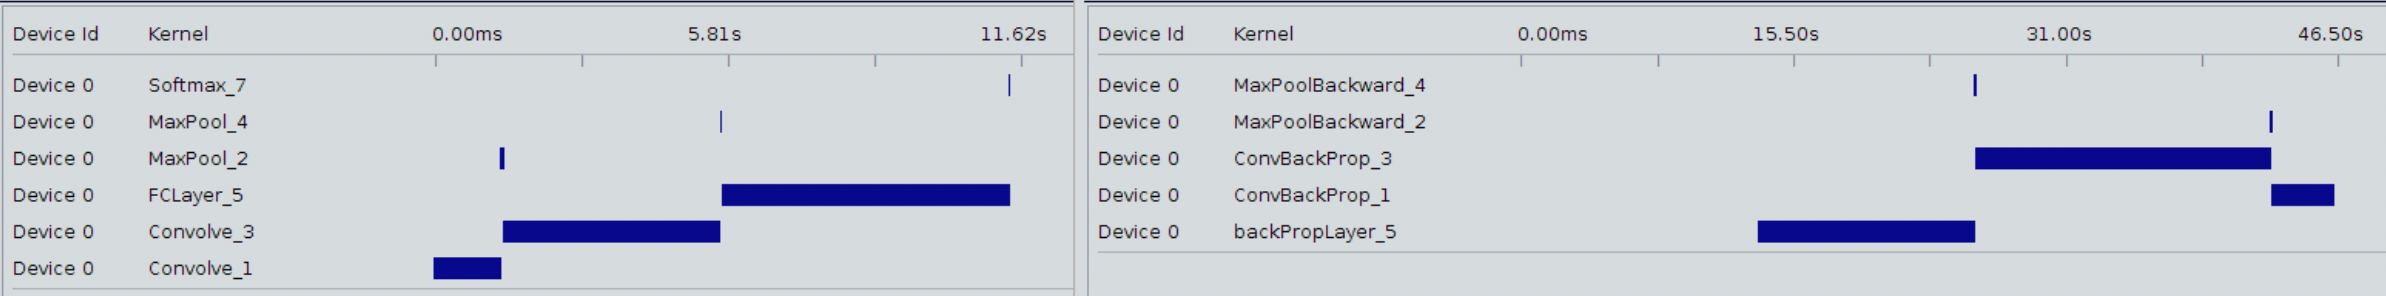
\includegraphics[width=1.0\textwidth]{Figures/fullprop}
\decoRule
\caption[fullprop]{ Dynamic Profiling results for minibatch on LeNet. }
\label{fig:fullprop}
\end{figure}

\begin{table}[]
\centering
\begin{tabular}{|c|c|c|c|}
\hline
\textbf{Batch Size} & \textbf{\begin{tabular}[c]{@{}c@{}}Total Epoch \\ Time\end{tabular}} & \textbf{\begin{tabular}[c]{@{}c@{}}Reconfiguration Time \\ (x2) in seconds\end{tabular}} & \textbf{\begin{tabular}[c]{@{}c@{}}$ \frac{Reconfiguration Time}{Total Epoch Time} $\end{tabular}} \\ \hline
1                   & 4.3                                                                  & 4.2                                                                                      & 97.6 \%                                                                                     \\ \hline
2048                & 49.1                                                                 & 4.6                                                                                      & 9.3\%                                                                                       \\ \hline
\end{tabular}
\caption{Reconfiguration Time Overhead}
\label{tab:reconfigure}
\end{table}


By looking at Fig. \ref{fig:fullprop} and after re-running the experiment time for multiple times, we realize that reconfiguration time is long and takes between 2 and 2.5 seconds in total. For a small batch size or in the case of a single image, reconfiguration time introduces a large overhead. When working with large batches, the effect is minimized ( as shown in Table \ref{tab:reconfigure} ). One iteration in the table consists of kernel reconfiguration ( twice ), forward propagation, and backward propagation with weight updates for the full batch.

In the case of a batch size of 2048, the overhead of reconfiguration is still large (9.7\%), however this is more feasible to perform as opposed to a single image. Nevertheless, with larger batch sizes, we risk reaching a local minimum when optimizing the loss function as discussed before in \ref{graddesc}.

\subsubsection{Challenges}

The implementation of LeNet required a lot of modifications until we started to see a decrease in the loss function. One of the challenges was the vanishing gradient problem \cite{hochreiter1998vanishing}. We solved this by replacing the ReLU function with the leaky ReLU which improved the training procedure. The Leaky ReLU function is given by \ref{lrelu}.
 \begin{equation}
  f(x) = \left\{
  \begin{array}{lr}
    x & : \textrm{if } x \ge 0 \\
    0.01x & : otherwise
  \end{array}
\right.
\label{lrelu}
 \end{equation}
 In back-propagating the error in the fully connected layers, we experimented with gradient clipping techniques which also improved the stability in the weight updates. 

We ran the batch size of 2048 on the FPGA, however it took as long as  ~2 hours per epoch and we did not get an improvement in accuracy. This may be due either to the batch size being too large, or because of some error introduced into the minibatch backpropagation implementation for convolutional layers. 

As for simply running Stochastic Gradient Descent,  it is unfeasible to run on the FPGA due to the overhead of reconfiguration which dominates runtime. Therefore, to test SGD, we used the Intel Emulator and noticed a decrease in the loss function but we did not run it until convergence as the emulator crashes when too many threads are launched and destroyed. 

\subsection{Simple Classifier}

\begin{table}[]
\centering
\begin{tabular}{|l|l|l|}
\hline
\textbf{Layer}           & \textbf{No. of Neurons} & \textbf{Trainable Parameters} \\ \hline
\textit{Input}           & 784 ( 28*28 )           & 0                             \\ \hline
\textit{Fully Connected} & 512                     & 401,920                       \\ \hline
\textit{Fully Connected} & 512                     & 262,656                       \\ \hline
\textit{Fully Connected} & 10                      & 5130                          \\ \hline
\textit{Softmax}         & 10                      & 0                             \\ \hline
\end{tabular}
\caption{Number of Trainable Parameters per Layer in the Simple Classifier.}
\label{tab:simplemod}
\end{table}

For additional verification, we compiled a simple neural network composed of only fully connected layers. The number of neurons per layer is shown in Table \ref{tab:simplemod}. We trained the model until convergence and unlike the LeNet model, both the full forward and backward propagation fit on the Arria 10 FPGA. 
It achieved reasonable runtime, $\approx$5.3 minutes per epoch and took 20 epochs to converge. We randomly sampled 5000 images of the MNIST Dataset for training and 500 images for testing. Eventually, the model achieved 67\% test error. 

In the simple model there is a \textbf{lot} of room to tune hyperparameters. Moreover, in this experiment, we did not aim to come up with the highest accuracy or fastest runtime.  The goal was to prove the correctness and the usability of the framework in a case where both forward and backward propagation fit on a single board configuration. Hopefully with a more advanced board, with a better fabric we can achieve better performance for more complex models.

%----------------------------------------------------------------------------------------
